\documentclass{article}
\usepackage[utf8]{inputenc}
\usepackage[margin=2cm]{geometry}
\usepackage{amsmath}
\usepackage{amssymb}
\usepackage{amsthm}
\usepackage{graphicx}
\usepackage{subfig}
\usepackage{enumitem}

\title{Mini-project 1 --- notes}
\author{Suzie Brown}
\date{\today}

%\usepackage[colorlinks=true, allcolors=blue]{hyperref}
\usepackage[round, sort&compress]{natbib}
\usepackage{har2nat} %%% Harvard reference style
\bibliographystyle{agsm}

\newcommand{\E}{\mathbb{E}}
\newcommand{\PR}{\mathbb{P}}
\newcommand{\V}{\operatorname{Var}}
\newtheorem{thm}{Theorem}

%% web reference for probabilistic analysis of some population models:
%% https://cs.nyu.edu/mishra/COURSES/09.HPGP/scribe2 (also see scribe 1,3,4)

%% web reference for deriving limit of (1-1/x)^x:
%% https://socratic.org/questions/how-do-you-find-the-limit-of-1-1-x-x-as-x-approaches-infinity

%% web reference for mean/variance number of steps to absorption of absorbing Markov chain:
%% https://en.wikipedia.org/wiki/Absorbing_Markov_chain#Expected_number_of_steps

\begin{document}
\section*{Kingman's $n$-coalescent}
From \citet{kingman1982gene} via \citet[Chapter 3]{wakeley2009} and \citet{mohle1998}.

In the notation of \citet{wakeley2009}, $T_i;\, i=2,\dots,n$ is the $i^{th}$ coalescence time, that is, the length of time for which there are exactly $i$ branches in the sample genealogy. The $n$-coalescent is the process in which these times are i.i.d.\ Exponentials:
\begin{equation*}
T_i \sim \operatorname{Exp}\left(\binom{i}{2}\right)
\end{equation*}
having
\begin{equation*}
\E(T_i) = \frac{2}{i(i-1)}, \qquad \V(T_i) = \left( \frac{2}{i(i-1)} \right)^2
\end{equation*}
By noting that the number of possible pairs from $i$ lineages is $\frac{i(i-1)}{2}$, the process can equivalently be formulated as a Poisson process where pairs of lineages coalesce independently at rate 1, with the pair to coalesce being chosen uniformly at random \citep[Section 3.2]{wakeley2009}.

\citet{mohle1998} writes the same process in terms of the infinitesimal generator $Q$ of a Markov process $\{R_r\}$ on the set of equivalence relations on $n$ elements, having entries
\begin{equation*}
q_{\xi\eta} =
\begin{cases}
-\frac{1}{2}b(b-1) &\text{if }\xi=\eta \\
1 & \text{if }\xi \prec\eta \\
0 & \text{otherwise}
\end{cases}
\end{equation*}
where $b$ is the number of equivalence classes of $\xi$, and $\xi \prec \eta$ means that $\eta$ is a state with exactly one more pair of lineages coalesced compared to $\xi$. [check this is equivalent to Wakeley's formulation]


\section*{Notes from \citet{mohle1998}}

\subsection*{Framework}
\begin{itemize}
\item Current generation is generation $0$; generations enumerated backward in time.
\item Generations are non-overlapping.
\end{itemize}

\subsection*{Notation}
\begin{description}
\item[$M_r$] population size at generation $r$
\item[$N := M_0$] initial population size
\item[$v_i^{(r)}$] (random) number of offspring of individual $i$ of generation $r$
\item[$n\leq N$] size of the sample of individuals in generation 0 to be considered
\item[$T_n$] the number of generations since the most recent common ancestor (MRCA) of the sample
\item[$\mathcal{R}_r$] the equivalence relation that contains the pair $(i,j)$ iff individuals $i$ and $j$ in the sample have a common ancestor in generation $r$
\item[$\{\mathcal{R}_r\}_{r\in\mathbb{N}}$] will be referred to as the \emph{ancestral process}
\item[$\Delta$] the minimal relation $\{(i,i); i=1,\dots,n\}$
\item[$\Theta$] the maximal relation $\{(i,j); i,j = 1,\dots,n\}$
\item[$p_{\xi\eta}(r)$] the transition probability $\PR(\mathcal{R}_r=\eta\mid\mathcal{R}_{r-1}=\xi)$ of the ancestral process
\item[$c_r$] the probability that a random pair of distinct individuals from generation $r$ have a common ancestor in generation $r-1$, called the \emph{coalescence probability}
\item[$\sigma^2(r)$] the expected \emph{mean crowding} of the offspring variables of generation $r$
\item[$X_r$] the number of descendants in generation $r$ in the forward genealogical process
\item[$\pi_{ij}(r)$] the transition probability $\PR(X_{r-1}=j\mid X_r=i)$ of the forward genealogical process
\item[$(x)_y$] denotes the descending factorial $x(x-1)\cdots(x-y+1)$
\end{description}

\subsection*{Assumptions}
\begin{enumerate}
\item\label{ass:gen_indep} $\{ v_1^{(r)},\dots,v_{M_r}^{(r)} \}$ is independent of $\{ v_1^{(s)},\dots,v_{M_s}^{(s)} \}$ for $r\neq s$
\item\label{ass:non_exch} $ v_1^{(r)},\dots,v_{M_r}^{(r)}$ are \textbf{not} assumed to be exchangeable
\end{enumerate}

\subsection*{Initial remarks}
\begin{enumerate}
\item From the definitions, we have that
\begin{equation}\label{eq:sum_vi}
\sum_{i=1}^{M_r} v_i^{(r)} = M_{r-1}
\end{equation}
\item Assumption \ref{ass:gen_indep} ensures that $\{\mathcal{R}_r\}_{r\in\mathbb{N}}$ is a Markov process (hence the applicability of transition probabilities).
\end{enumerate}

\subsection*{Calculating the coalescence rate}
A combinatorial argument allows us to derive an expression for the transition probability $p_{\xi\eta}(r)$ of the ancestral process:
\begin{equation}\label{eq:trans_prob}
p_{\xi\eta}(r) = \frac{1}{(M_{r-1})_b} \sum_{\substack{i_1,\dots,i_a =1 \\ \text{distinct}}}^{M_r} \E\left[(v_{i_1}^{(r)})_{b_1}\cdots (v_{i_a}^{(r)})_{b_a}\right]
\end{equation}
The sum is over all the possible ordered choices of the $a$ parents from generation $r$. Inside the sum is the expected number of ways to have at least the required number of offspring from each parent, given this choice of parents. Thus the whole sum represents the probability of finding a set of parents that produce the required number of offspring. Then dividing by the number of ordered ways to choose $b$ offspring from generation $r-1$ ensures that the parents produce the \emph{correct} ordered offspring. Overall then we have the probability that exactly the right subsets of offspring from generation $r-1$ coalesce in generation $r$, counting all the different parents to which they could coalesce.

In the special case where $ v_1^{(r)},\dots,v_{M_r}^{(r)}$ are exchangeable, it is not necessary to have separate terms for different combinations of individuals $i_1,\dots,i_a$, so \eqref{eq:trans_prob} simplifies to
\begin{equation}\label{eq:trans_prob_exch}
p_{\xi\eta}(r) = \frac{(M_r)_a}{(M_{r-1})_b} \E\left[(v_{1}^{(r)})_{b_1}\cdots (v_{a}^{(r)})_{b_a}\right]
\end{equation}

Now let us consider the coalescence time $T_n$. In general we have $\PR(T_n>l)=\PR(\mathcal{R}_l \neq \Theta)$. In the case $n=2$ (i.e.\ time to coalescence for a pair of individuals), we can say something further:
\begin{align}
\PR(T_2>l) &= \PR(\mathcal{R}_l = \Delta) \notag\\
&= \prod_{r=1}^l p_{\Delta\Delta}(r) \notag\\
&= \prod_{r=1}^l \frac{1}{(M_{r-1})_2} \sum_{i=1}^{M_r} \sum_{j \neq i} \E\left[v_i^{(r)}v_j^{(r)}\right] \notag\\
&= \prod_{r=1}^l \frac{1}{(M_{r-1})_2} \sum_{i=1}^{M_r} \E\left[v_i^{(r)}\sum_{j \neq i}v_j^{(r)}\right] \notag\\
&= \prod_{r=1}^l \frac{1}{(M_{r-1})_2} \sum_{i=1}^{M_r} \E\left[v_i^{(r)}(M_{r-1}-v_i^{(r)})\right] \\
&= \prod_{r=1}^l \frac{1}{(M_{r-1})_2} \left\{ \E \left[M_{r-1}\sum_{i=1}^{M_r}v_i^{(r)}\right]  - \sum_{i=1}^{M_r} \E \left[(v_i^{(r)})^2\right]\right\} \notag\\
&= \prod_{r=1}^l \frac{1}{(M_{r-1})_2} \left\{ \E \left[M_{r-1}^2\right]  - \sum_{i=1}^{M_r} \E \left[(v_i^{(r)})^2\right]\right\} \notag\\
&= \prod_{r=1}^l \frac{1}{(M_{r-1})_2} \left\{M_{r-1}(M_{r-1}-1) + \sum_{i=1}^{M_r} \E \left[v_i^{(r)}\right]  - \sum_{i=1}^{M_r} \E \left[(v_i^{(r)})^2\right]\right\} \notag\\
&= \prod_{r=1}^l \frac{1}{(M_{r-1})_2} \left\{M_{r-1}(M_{r-1}-1) + \sum_{i=1}^{M_r} \E \left[v_i^{(r)} - (v_i^{(r)})^2\right]\right\} \notag\\
&= \prod_{r=1}^l \frac{1}{(M_{r-1})_2} \left\{M_{r-1}(M_{r-1}-1) - \sum_{i=1}^{M_r} \E \left[v_i^{(r)}(v_i^{(r)}-1)\right]\right\} \notag\\
&= \prod_{r=1}^l \frac{1}{(M_{r-1})_2} \left\{ (M_{r-1})_2 - \sum_{i=1}^{M_r} \E \left[(v_i^{(r)})_2\right]\right\} \notag\\
&= \prod_{r=1}^l \left\{ 1- \frac{1}{(M_{r-1})_2}  \sum_{i=1}^{M_r} \E \left[(v_i^{(r)})_2\right]\right\} \label{eq:coal_prob_prod}
\end{align}
Now we have $\PR(T_2>l)$ in the form $\prod (1-c_r)$, where $c_r$ represents the \emph{coalescence probability}, i.e.\ the probability that a randomly chosen pair of (distinct) individuals from generation $r-1$ have a common ancestor in generation $r$.
We can derive an equivalent expression for the coalescence probability, $c_r= \sigma^2(r) / (M_{r-1}-1)$, where $\sigma^2(r)$ is the expected \emph{mean crowding} of the offspring variables $\{ v_1^{(r)},\dots,v_{M_r}^{(r)} \}$.
\begin{align}
c_r &= \frac{1}{(M_{r-1})_2} \sum_{i=1}^{M_r} \E \left[ (v_i^{(r)})_2 \right] \label{eq:coal_prob1}\\
&= \frac{1}{M_{r-1}-1} \frac{1}{M_{r-1}} \E \left[ \sum_{i=1}^{M_r} (v_i^{(r)})_2 \right] \notag\\
&= \frac{1}{M_{r-1}-1} \frac{1}{\E[M_{r-1}]} \E \left[ \sum_{i=1}^{M_r} (v_i^{(r)})_2 \right] \notag\\
&= \frac{1}{M_{r-1}-1} \frac{1}{\E[ \sum_{i=1}^{M_r} v_i^{(r)}]} \E \left[ \sum_{i=1}^{M_r} (v_i^{(r)})_2 \right] \notag\\
&= \frac{1}{M_{r-1}-1} \E \left[  \frac{\sum_{i=1}^{M_r} (v_i^{(r)})_2}{\sum_{i=1}^{M_r} v_i^{(r)}}  \right] \label{eq:coal_prob2}
\end{align}


\subsection*{Example: generalised Wright-Fisher model}
Model as Wright-Fisher, except we don't assume exchangeability of offspring distributions. Instead of choosing parents multinomially with equal weights, we choose them multinomially with unequal weights. 
Thus the marginal offspring distributions are 
$v_i^{(r)} \sim \operatorname{Bin}(M_{r-1}, p_i)$.
We therefore have $\E(v_i^{(r)}) = M_{r-1}p_i$ and $\E(v_i^{(r)}2) = M_{r-1}p_i(1-p_i+M_{r-1}p_i)$. Hence
\begin{align*}
c_r &= \frac{1}{(M_{r-1})_2} \sum_{i=1}^{M_r} \E[(v_i^{(r)})_2] \\
&= \frac{1}{(M_{r-1})_2} \sum_{i=1}^{M_r} \E[v_i^{(r)}2 - v_i^{(r)}] \\
&= \frac{1}{(M_{r-1})_2} \sum_{i=1}^{M_r} [M_{r-1}p_i (1-p_i + M_{r-1}p_i -1 )] \\
&= \frac{1}{(M_{r-1})_2} \sum_{i=1}^{M_r} [M_{r-1}p_i^2 (M_{r-1} -1 )] \\
&= \frac{1}{(M_{r-1})_2} \sum_{i=1}^{M_r} [(M_{r-1})_2 p_i^2] \\
&= \sum_{i=1}^{M_r} p_i^2
\end{align*}
and
\begin{align*}
\sigma^2(r) &= \frac{1}{M_{r-1}} \sum_{i=1}^{M_r} \E[(v_i^{(r)})_2] \\
&= (M_{r-1}-1)\sum_{i=1}^{M_r} p_i^2
\end{align*}

\subsubsection*{Special case: uniform weights}
Suppose $p_i = 1/M_r$ for all $i$ (the standard Wright-Fisher model).
Then we have
\begin{equation*}
c_r = \sum_{i=1}^{M_r} p_i^2 = \sum_{i=1}^{M_r} \frac{1}{M_r^2} = \frac{1}{M_r} 
\end{equation*}
and if the population size doesn't depend on $r$ (i.e.\ $M_r \equiv N$), we can find the full distribution of $T_2$:
\begin{equation*}
\PR(T_2 >l) = \prod_{r=1}^{l} (1-c_r) = \prod_{r=1}^l \left(1- \frac{1}{M_r}\right) = \left(1 - \frac{1}{N}\right)^l
\end{equation*}
% ERM......... SOMETHING FISHY HERE
and deduce
\begin{equation*}
\E [T_2] = \sum_{l=0}^\infty \PR(T_2 >l) = \sum_{l=0}^\infty (1-c_r)^l = c^{-1} = M_r = N
\end{equation*}
A realisation of 12 generations of this model with $N=10$ is shown in Figure \ref{fig:eg_WF}.
\begin{figure}
\centering
\subfloat[][]{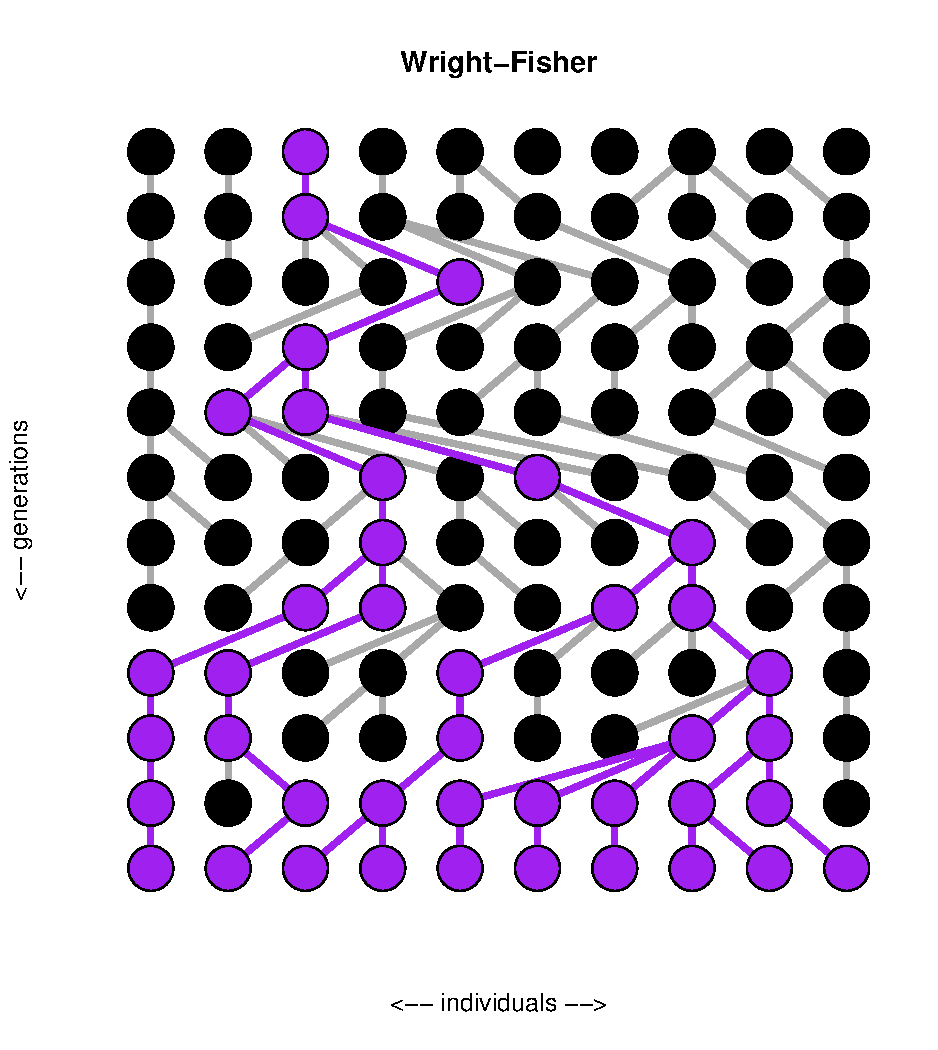
\includegraphics[width=0.5\textwidth]{eg_WF.pdf}\label{fig:eg_WF}}
\subfloat[][]{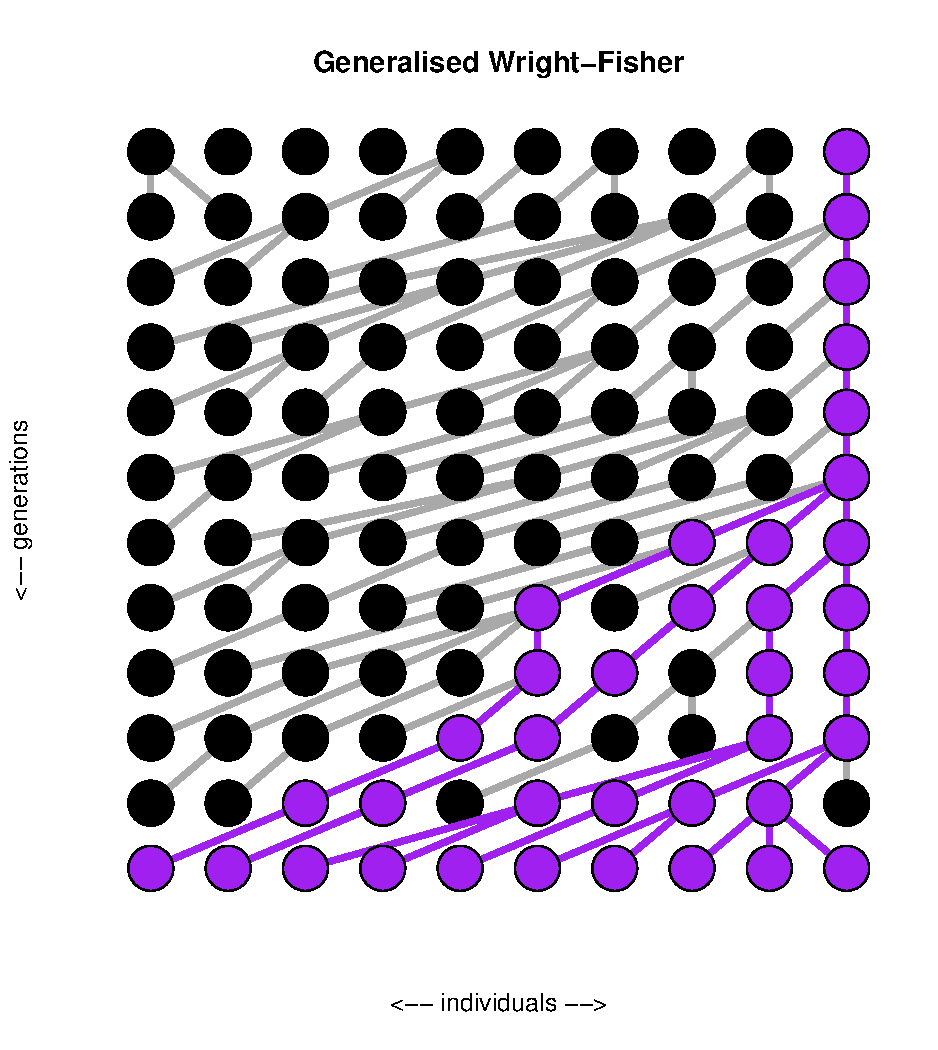
\includegraphics[width=0.5\textwidth]{eg_genWF.pdf}\label{fig:eg_genWF}}
\caption{Realisations from a Wright-Fisher model with $N=10$ individuals and 12 generations. (a) is from the standard model with uniform weights (``fitnesses''). (b) is from the generalised model with weighting on individual $i$ proportional to $i$.}
\end{figure}

\subsubsection*{Special case: linearly increasing weights}
Suppose $p_i = 2i/(M_r(M_r-1))$ for each $i$. Then
\begin{equation*}
c_r = \sum_{i=1}^{M_r} p_i^2 = \sum_{i=1}^{M_r} \frac{4i^2}{M_r^2(M_r+1)^2} = \frac{4}{M_r^2(M_r+1)^2} \sum_{i=1}^{M_r} i^2 = \frac{2(2M_r+1)}{3M_r(M_r+1)}
\end{equation*}
and for constant population size
\begin{equation*}
\E [T_2] = \frac{3N(N+1)}{2(2N+1)}
\end{equation*}
A realisation of 12 generations of this model with $N=10$ is shown in Figure \ref{fig:eg_genWF}.


\subsection*{The theorem of M\"ohle}
\subsubsection*{Algebraic tools for proof}
Here are a few identities and inequalities that will be referred to when proving the theorem. \eqref{eq:tools_swap_sum_prod} is obtained using a multinomial expansion, \eqref{eq:tools_bernoulli_ineq} using Bernoulli's inequality, and \eqref{eq:tools_power_v_fact}--\eqref{eq:tools_fact_asymp2} by expanding factorials. 
\begin{align}
& \sum_{i_1\dots i_m = 1}^n \prod_{j=1}^m x_{i_j} = \prod_{j=1}^m \sum_{i=1}^n x_i = \left( \sum_{i=1}^n x_i \right)^m \label{eq:tools_swap_sum_prod}\\
& (k-x)^n = k^n\left(1-\frac{x}{k}\right)^n \leq k^n - nxk^{n-1} \label{eq:tools_bernoulli_ineq}\\
& n^a \geq (n)_a \label{eq:tools_power_v_fact}\\
%& (n)_a = (n)_b (n-b)_{a-b} \text{, if } 0\leq b\leq a \label{eq:tools_fact_take_two}\\
& (n)_a \leq (n)_b \,n^{a-b} \text{, if } 0\leq b\leq a \label{eq:tools_fact_taketwo_bd}\\
& \frac{n^{a-b}}{(n)_a} = \frac{1}{(n)_b} + O(n^{-b-1}) \label{eq:tools_fact_asymp1}\\
& \frac{1}{(n)_b} = \frac{1}{n^b} + O(n^{-b-1}) \label{eq:tools_fact_asymp2}
\end{align}

Now for simplicity we assume a constant population size $M_r \equiv N$, which for the purposes of SMC will generally be satisfied.
\begin{thm}
Let $T \subset \mathbb{R}$ and suppose there is a function $\tau : T \to \mathbb{N}_0$ satisfying:
\begin{enumerate}[label=(\Alph*)]
\item\label{assn:coal_rate} correct limiting coalescence rate
\begin{equation*}
\forall t \in T, \,\lim_{N\to\infty} \sum_{r=1}^{\tau(t)} c_r =t
\end{equation*}

\item\label{assn:coal_var} variance of coalescence rate goes to zero
\begin{equation*}
\forall t \in T, \,\lim_{N\to\infty} \sum_{r=1}^{\tau(t)} c_r^2 =0
\end{equation*}

\item\label{assn:triple_coal} no triple coalescences
\begin{equation*}
\forall t \in T, \forall k\in\mathbb{N}_0,\, \lim_{N\to\infty} \sup_{r\leq\tau(t)} \frac{1}{N^3 c_r} \sum_{i=1}^N \E\left[ (v_i^{(r)})_2 (v_i^{(r)})^k \right] =0
\end{equation*}

\item\label{assn:multi_coal} only one coalescence at a time
\begin{equation*}
\forall t \in T,\, \lim_{N\to\infty} \sup_{r\leq\tau(t)} \frac{1}{N^4 c_r} \sum_{i,j=1}^N \E\left[ (v_i^{(r)})_2 (v_j^{(r)})^2 \right] =0
\end{equation*}
\end{enumerate}
Then the finite-dimensional distributions of $\{\mathcal{R}_{\tau(t)}\}_{t\in T}$ converge to those of the $n$-coalescent (with time restricted to $T$) in the limit $N\to\infty$.
\end{thm}
Note that, since (being a probability) $c_r \geq 0$ for all $r$; under \ref{assn:coal_rate}, \ref{assn:coal_var} is equivalent to
\begin{equation}
\forall t \in T,\, \lim_{N\to\infty} \sup_{r\leq\tau(t)} c_r =0
\end{equation}

\begin{proof}
We first bound the transition probability $p_{\xi\eta}(r)$ as given by \eqref{eq:trans_prob}, in each of four possible cases. This will show that the only type of coalescence event to occur at any one time in the limit $N\to\infty$ is a merger of exactly one pair of lineages (\ref{case:pair_merge} below). 
Assume the offspring numbers $v_i^{(r)}$ are known (so we drop the expectations).
\begin{enumerate}[label = \textbf{Case \arabic*.}]
\item\label{case:pair_merge} $\eta$ is obtained from $\xi$ by merging exactly one pair of lineages, i.e.\ $b_1=2, b_2=\dots=b_a=1$, and $b=a+1$. We derive an upper bound:
\begin{align}
p_{\xi\eta}(r) &= \frac{1}{(N)_b} \sum_{\substack{i_1,\dots,i_a =1 \\ \text{distinct}}}^{N} (v_{i_1}^{(r)})_2(v_{i_2}^{(r)})_1\cdots (v_{i_a}^{(r)})_1 &\notag\\
&\leq \frac{1}{(N)_b} \sum_{i_1,\dots,i_a=1}^N (v_{i_1}^{(r)})_2 (v_{i_2}^{(r)})_1 \cdots (v_{i_a}^{(r)})_1 &\text{dropping distinctness} \notag\\
&= \frac{1}{(N)_b} \sum_{i=1}^N (v_i^{(r)})_2 \sum_{i_2,\dots,i_a=1}^N v_{i_2}^{(r)} \cdots v_{i_a}^{(r)} & \notag\\
&= \frac{1}{(N)_b} \sum_{i=1}^N (v_i^{(r)})_2 (v_1^{(r)} + \dots + v_N^{(r)})^{a-1} & \text{using \eqref{eq:tools_swap_sum_prod}} \notag\\
&= \frac{N^{b-2}}{(N)_b} \sum_{i=1}^N (v_i^{(r)})_2 & \text{using \eqref{eq:sum_vi}} \notag\\
&= \left( \frac{1}{(N)_2} + O(N^{-3}) \right) \sum_{i=1}^N (v_i^{(r)})_2 & \text{using \eqref{eq:tools_fact_asymp1}} \label{eq:case1_upper}\\
&= c_r + o(c_r) & \text{by \eqref{eq:coal_prob1} and \ref{assn:triple_coal}} \notag
\end{align}
and a lower bound:
\begin{align}
p_{\xi\eta}(r) &= \frac{1}{(N)_b} \sum_{\substack{i_1,\dots,i_a =1 \\ \text{distinct}}}^{N} (v_{i_1}^{(r)})_2(v_{i_2}^{(r)})_1\cdots (v_{i_a}^{(r)})_1 &\notag\\
&= \frac{1}{(N)_b} \sum_{i=1}^N (v_i^{(r)})_2 \sum_{\substack{i_2,\dots,i_a =1 \\ \text{distinct} \neq i }}^{N} (v_{i_2}^{(r)})_1\cdots (v_{i_a}^{(r)})_1 &\notag\\
&\geq \frac{1}{(N)_b} \sum_{i=1}^N (v_i^{(r)})_2 \sum_{j\neq i} \sum_{\substack{i_3,\dots,i_a\\ \neq i}}\left[ v_j\cdot v_{i_3}\cdots v_{i_a} - \binom{b-2}{2}(v_j^{(r)})^2 \cdot v_{i_4}\cdots v_{i_a} \right] & \label{eq:transprob_lowerbd}\\
&= \frac{1}{(N)_b} \sum_{i=1}^N (v_i^{(r)})_2 \left[ \sum_{i_2,\dots,i_a\neq i} v_{i_2}\cdots v_{i_a} - \binom{b-2}{2} \sum_{i_3,\dots,i_a\neq i} v_{i_3}\cdots v_{i_a} \sum_{j \neq i} (v_j^{(r)})^2 \right] & \notag\\
&= \frac{1}{(N)_b} \sum_{i=1}^N (v_i^{(r)})_2 \left[ (N-v_i)^{b-2} - \binom{b-2}{2} \sum_{j\neq i} (v_j^{(r)})^2 N^{b-4} \right] &\text{using \eqref{eq:tools_swap_sum_prod}} \notag\\
&= \frac{1}{(N)_b} \sum_{i=1}^N (v_i^{(r)})_2  (N-v_i)^{b-2} - \frac{1}{(N)_b} \binom{b-2}{2} \sum_{i\neq j=1}^{N} (v_i^{(r)})_2 (v_j^{(r)})^2 N^{b-4} & \notag\\
&\geq \frac{1}{(N)_b} \sum_{i=1}^N (v_i^{(r)})_2  (N)^{b-2} - \frac{1}{(N)_b}(b-2)\sum_{i=1}^{N} (v_i^{(r)})_2 v_i^{(r)} N^{b-3} \notag\\
&\phantom{=\qquad\qquad} - \frac{1}{(N)_b}\binom{b-2}{2} \sum_{i\neq j=1}^{N} (v_i^{(r)})_2 (v_j^{(r)})^2 N^{b-4} &\text{using \eqref{eq:tools_bernoulli_ineq}} \notag\\
&\geq \frac{1}{(N)_2} \sum_{i=1}^N (v_i^{(r)})_2 - \frac{(b-2)N^{b-3}}{(N)_b}\sum_{i=1}^{N} (v_i^{(r)})_2 v_i^{(r)} \notag\\
&\phantom{=\qquad\qquad} -\frac{N^{b-4}}{(N)_b}\binom{b-2}{2} \sum_{i\neq j=1}^{N} (v_i^{(r)})_2 (v_j^{(r)})^2 & \notag\\
&= \frac{1}{(N)_2} \sum_{i=1}^N (v_i^{(r)})_2 - \left[\frac{(b-2)}{N^3} +O(N^{-4}) \right] \sum_{i=1}^{N} (v_i^{(r)})_2 v_i^{(r)} \notag\\
&\phantom{=\qquad\qquad} -\left[ \frac{1}{N^4}\binom{b-2}{2} + O(N^{-5}) \right] \sum_{i\neq j=1}^{N} (v_i^{(r)})_2 (v_j^{(r)})^2 &\text{using \eqref{eq:tools_fact_asymp1}, \eqref{eq:tools_fact_asymp2}} \\
&= c_r + o(c_r) &\text{by \eqref{eq:coal_prob1},\ref{assn:triple_coal},\ref{assn:multi_coal}} \notag
\end{align}
Hence in this case $p_{\xi\eta}(r)=c_r +o(c_r)$.
The inequality \eqref{eq:transprob_lowerbd} is obtained by bounding the number of configurations with distinct parents by the the number of configurations with not necessarily distinct parents minus the number with at least one pair of parents chosen indistinctly. This leaves us with only the distinct-parents configurations since all indistinct choices must necessarily have a pair of parents chosen indistinctly, and the inequality arises from double-counting.

\item\label{case:triple_merge} $\eta$ is obtained from $\xi$ by merging three or more lineages into one, possibly as well as other simultaneous mergers, i.e.\ $b_1\geq3$.
\begin{align}
p_{\xi\eta}(r) &= \frac{1}{(N)_b} \sum_{\substack{i_1,\dots,i_a =1 \\ \text{distinct}}}^{N} (v_{i_1}^{(r)})_{b_1}(v_{i_2}^{(r)})_{b_2}\cdots (v_{i_a}^{(r)})_{b_a} &\notag\\
&\leq \frac{1}{(N)_b} \sum_{i=1}^{N} (v_{i}^{(r)})_{b_1} \sum_{i_2,\dots,i_a =1}^{N} (v_{i_2}^{(r)})_{b_2}\cdots (v_{i_a}^{(r)})_{b_a} &\notag\\
&\leq \frac{1}{(N)_b} \sum_{i=1}^{N} (v_{i}^{(r)})_{b_1} (v_1^{(r)}+\dots+v_a^{(r)})^{b_2+\dots+b_a} &\text{using \eqref{eq:tools_swap_sum_prod}} \notag\\
&\leq \frac{1}{(N)_b} \sum_{i=1}^{N} (v_{i}^{(r)})_{b_1} N^{b-3} &\text{since }b_2+\dots+b_a\leq b-3 \label{eq:triplemerge_bound_spinoff}\\
%%^ HAVE TO SPIN OFF HERE FOR KJJS PROOF
&\leq \frac{N^{b-3}}{(N)_b} \sum_{i=1}^{N} (v_{i}^{(r)})_{2}(v_{i}^{(r)})^{b_1-2}  &\text{using \eqref{eq:tools_fact_taketwo_bd}} \\
&= o(c_r) &\text{using \ref{assn:triple_coal}} \notag
\end{align}

\item\label{case:multi_merge} $\eta$ is obtained from $\xi$ via two or more pair mergers, with no merges of more than two lineages, i.e.\ $2=b_1=b_2\geq b_3\geq\dots\geq b_a\geq1$.
\begin{align}
p_{\xi\eta}(r) &= \frac{1}{(N)_b} \sum_{\substack{i_1,\dots,i_a =1 \\ \text{distinct}}}^{N} (v_{i_1}^{(r)})_2 (v_{i_2}^{(r)})_2 (v_{i_3}^{(r)})_{b_3}\cdots (v_{i_a}^{(r)})_{b_a} &\notag\\
&\leq \frac{1}{(N)_b} \sum_{i=1}^{N} (v_{i}^{(r)})_2 \sum_{j=1}^N (v_j^{(r)})_2 \sum_{i_3,\dots,i_a =1}^{N} (v_{i_3}^{(r)})_{b_3}\cdots (v_{i_a}^{(r)})_{b_a} &\text{dropping distinctness}\notag\\
&\leq \frac{1}{(N)_b} \sum_{i=1}^{N} (v_{i}^{(r)})_2 \sum_{j=1}^N (v_j^{(r)})^2 \sum_{i_3,\dots,i_a =1}^{N} (v_{i_3}^{(r)})_{b_3}\cdots (v_{i_a}^{(r)})_{b_a} &\text{using \eqref{eq:tools_power_v_fact}} \notag\\
&\leq \frac{1}{(N)_b} \sum_{i,j=1}^{N} (v_{i}^{(r)})_2 (v_j^{(r)})^2 (v_1^{(r)}+\dots+v_N^{(r)})^{b_3+\dots +b_a} &\notag\\
&=\frac{N^{b-4}}{(N)_b} \sum_{i,j=1}^N (v_{i}^{(r)})_2 (v_j^{(r)})^2 & \\
&= o(c_r) &\text{using \ref{assn:multi_coal}} \notag
\end{align}

\item\label{case:no_change} $\eta=\xi$, i.e.\ $b_1=\dots=b_a=1$, and $a=b$.
\begin{align}
p_{\xi\xi}(r) &= \frac{1}{(N)_a} \sum_{\substack{i_1,\dots,i_a =1 \\ \text{distinct}}}^{N} (v_{i_1}^{(r)})_1  \cdots (v_{i_a}^{(r)})_1 & \notag\\
&= \frac{1}{(N)_a} \sum_{\substack{i_1,\dots,i_a =1 \\ \text{distinct}}}^{N} v_{i_1}^{(r)} \cdots v_{i_a}^{(r)} & \notag\\
&= \frac{1}{(N)_a} \left[ \sum_{i_1,\dots,i_a =1}^N v_{i_1}^{(r)} \cdots v_{i_a}^{(r)} - \binom{a}{2}\sum_{j=1}^N (v_j^{(r)})^2 \sum_{i_3,\dots,i_a =1}^N v_{i_3}^{(r)} \cdots v_{i_a}^{(r)} \right] &\label{eq:transprob_lowerbd2}\\
&= \frac{1}{(N)_a} \left[ (v_1^{(r)}+\dots+v_N^{(r)})^a - \binom{a}{2} \sum_{i=1}^N (v_i^{(r)})^2 (v_1^{(r)}+\dots+v_N^{(r)})^{a-2} \right] &\text{using \eqref{eq:tools_swap_sum_prod}} \notag\\
&= \frac{1}{(N)_a} \left[ N^a - \binom{a}{2} N^{a-2} \sum_{i=1}^N (v_i^{(r)})^2 \right] &\notag\\
&\geq 1- \binom{a}{2} \frac{N^{a-2}}{(N)_a} \sum_{i=1}^N (v_i^{(r)})^2 &\text{using \eqref{eq:tools_power_v_fact}}\notag\\
%&= 1- \binom{a}{2} \frac{N^{a-2}}{(N)_2 (N-2)_{a-2}} \sum_{i=1}^N (v_i^{(r)})^2 &\text{using \eqref{eq:tools_fact_take_two}}\notag\\
&= 1- \binom{a}{2} \left[ \frac{1}{(N)_2} + O(N^{-3}) \right] \sum_{i=1}^N (v_i^{(r)})^2 &\text{using \eqref{eq:tools_fact_asymp1}}\\
&= 1- c_r +o(c_r) &\notag
\end{align}
\end{enumerate}
The equality \eqref{eq:transprob_lowerbd2} is obtained in the same way as \eqref{eq:transprob_lowerbd}, with no double-counting.
We have now shown that the only coalescence events having positive probability in the limit $N\to\infty$ are staying the same (\ref{case:no_change}) or merging a single pair of lineages (\ref{case:pair_merge}). All other possibilities have asymptotic probability $o(c_r)$.

It remains to show that the finite-dimensional distributions converge to those of the Kingman coalescent. Because the processes considered are Markov even when viewed as coalescing backwards in time, it suffices to show that the generators of the process converge to the generators of the Kingman coalescent (this will no longer be the case for the processes considered in \citet{koskela2018}).
\end{proof}

For the argument of \citet{koskela2018}, a different form is needed for the upper bound on triple mergers (\ref{case:triple_merge}). Starting from \eqref{eq:triplemerge_bound_spinoff}, we obtain:
\begin{align}
p_{\xi\eta}(r) &\leq \frac{1}{(N)_b} \sum_{i=1}^{N} (v_{i}^{(r)})_{b_1} N^{b-3} \notag\\
&\leq \frac{N^{b-3}}{(N)_b} \sum_{i=1}^{N} (v_{i}^{(r)})^{b_1} \notag\\
&= \left[ \frac{1}{N^3} + O(N^{-4}) \right] \sum_{i=1}^{N} (v_{i}^{(r)})^{b_1}
\end{align}



\section*{Coalescence in the Moran and Wright-Fisher models}
The results in this section come from my own reasoning and investigation, though I'm sure that they can (if correct) be found somewhere else.

\subsection*{Moran model}
We would like to know about the distribution of the \emph{full coalescence time} $\tau$, the first generation backwards in time at which all $N$ individuals in generation 0 have coalesced.
Let us consider the process by which coalescence occurs in the Moran model.

\subsubsection*{The appearance of an absorbing Markov chain}
In any one generation, at most one pair can coalesce (alternatively, the same individual dies and gives birth so nothing changes). However, a pair coalescence does not always represent a coalescence in the ancestry of interest, i.e.\ the ancestral line of the $N$ generation-0 individuals. 
We denote by $c_r$ the number of ``useful'' pair coalescences that have happened up to and including generation $r$. Thus $c_0=0$. Note that the maximum value of $c_r$ is $N-1$ (indicating that all $N$ lineages have coalesced and the MRCA has been reached). It is also evident that $N-c_r$ gives the number of individuals in generation $r$ that are part of a lineage continuing to generation 0. 

The crucial observation is that a pair coalescence corresponds to a coalescence in the $N$ lineages of interest (increasing the value of $c_r$ by 1) if and only if the pair consist of two distinct ``useful'' individuals out of these $N-c_r$.
Since $c_{r+1}$ depends only on $N$ and $c_r$, $\{c_r\}_{r\in\mathbb{N}}$ is a Markov chain, with state space $\{0, \dots, N-1\}$, absorbing state $N-1$ and transition probabilities derived below.

The first time (backwards in time) that a pair coalesces will always be useful, since all $N$ individuals are useful. Thus the probability $\PR(c_{r+1} = 1 \mid c_r =0)$ is simply the probability of choosing two \emph{distinct} individuals from generation $r-1$.
\begin{equation*}
p_{0,1} := \PR(c_{r+1} = 1 \mid c_r =0) = \frac{N}{N}\frac{N-1}{N} = 1-\frac{1}{N}
\end{equation*}
Now consider the transition probabilities from a general state i.
Given $c_{r}=i$, $c_{r+1}$ can take only the values $i$ or $i+1$. To increase by 1, we must have a useful pair coalescence. Thus the probability $\PR(c_{r+1} = i+1 \mid c_r =i)$ is the probability of choosing two distinct individuals from the $N-i$ useful individuals.
\begin{equation*}
p_{i,i+1} := \PR(c_{r+1} = i+1 \mid c_r =i) = \frac{N-i}{N}\frac{N-i-1}{N} \qquad i=1,\dots,N-2
\end{equation*}
and we see that the expression for $p_{0,1}$ was a special case of this.
The probability of staying in state $i$ will be $p_{i,i} = 1-p_{i,i+1}$ for $i=1,\dots,N-2$. The Markov chain is now fully specified:
\begin{equation}\label{eq:moran_coal_transprob}
p_{i,j} := \PR(c_{r+1} = j \mid c_r =i) = 
\begin{cases}
  1 &\text{if } i=j=N-1 \\
  1-\frac{(N-i)(N-i-1)}{N^2} &\text{if } j=i;\, i=0,\dots,N-2 \\
  \frac{(N-i)(N-i-1)}{N^2} &\text{if } j=i+1;\, i=0,\dots,N-2 \\
  0 &\text{otherwise}
\end{cases}
\end{equation}
Now let us return to the quantity of interest $\tau$, which is the time to absorption of this Markov chain.
we use without proof the following results about absorbing Markov chains.
Let $Q$ be the part of the transition matrix $P$ containing only transition probabilities between transient states (in this case the first $N-2$ rows and columns of $P$). Define $R := (I-Q)^{-1}$.
Then $\E (\tau \mid c_0=i)$ is given by the $i^{th}$ entry of $t:=R\mathbf{1}$, and $\V(\tau \mid c_0=i)$ is given by the $i^{th}$ entry of $(2R-I)t-t^2$, where $t^2$ is the element-wise square of $t$. Our chain starts at 0, so we take the corresponding entry to find $\E(\tau)$ and $\V(\tau)$.

We can easily calculate these quantities numerically for any fixed $N$. Figure \ref{fig:moran_coal} shows the behaviour of $\E(\tau)$ over a range of population sizes $N$. It seems that when $\tau$ is measured in rescaled generations, its expectation is linear in $N$. Can we prove this analytically? We see a similar story in the standard deviation of $\tau$ under rescaling, although the relationship appears to be linear only asymptotically. Can we prove this analytically?
%% perhaps we can use the special properties of the chain (i.e. only +0 and +1 steps possible) to derive some stronger properties --- the full distribution of tau???
\begin{figure}
  \centering
  \subfloat[][]{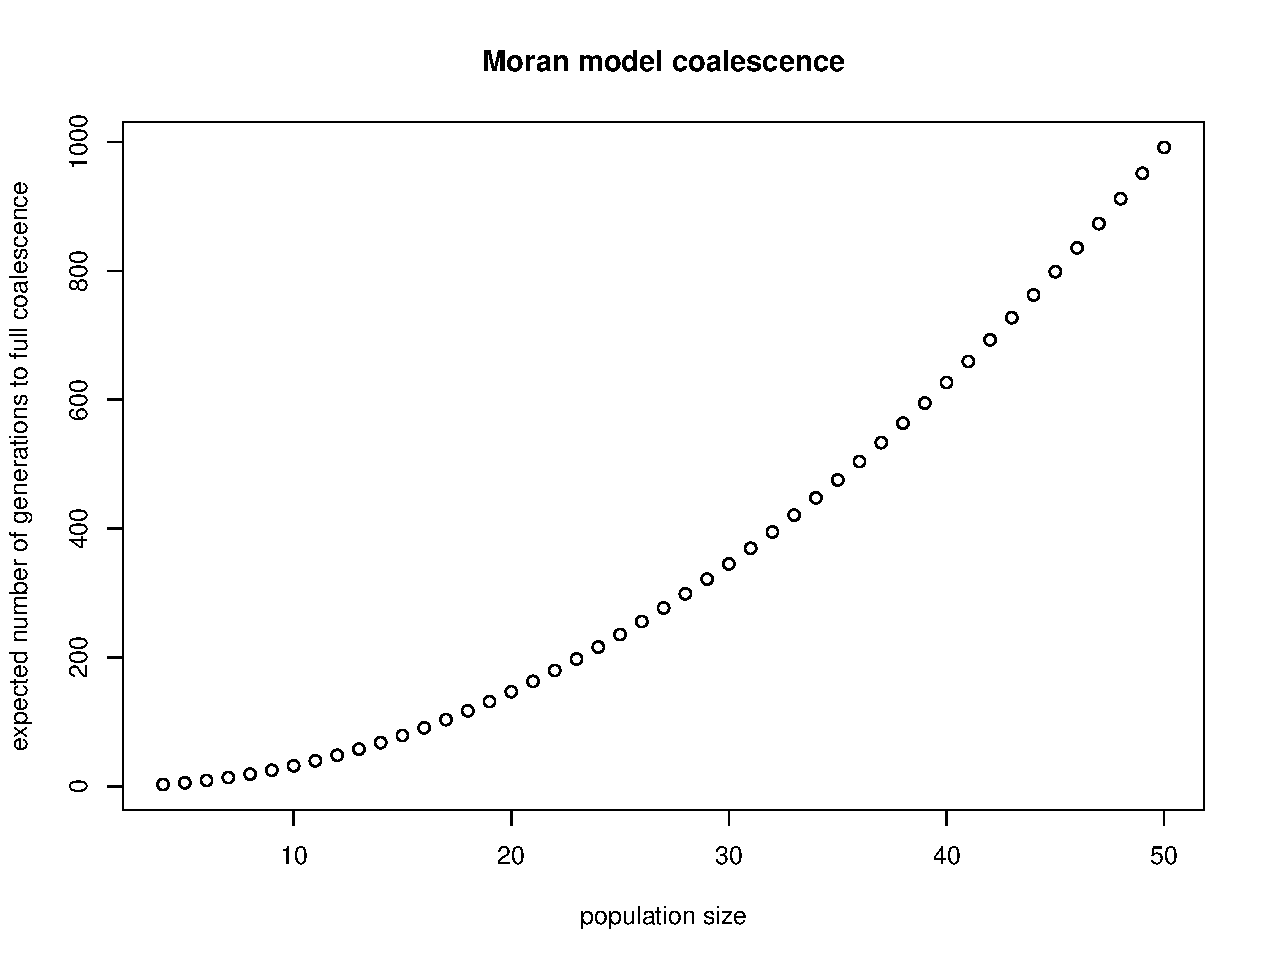
\includegraphics[width=0.5\textwidth]{moran_fullcoal.pdf}\label{fig:moran_fullcoal}}
  \subfloat[][]{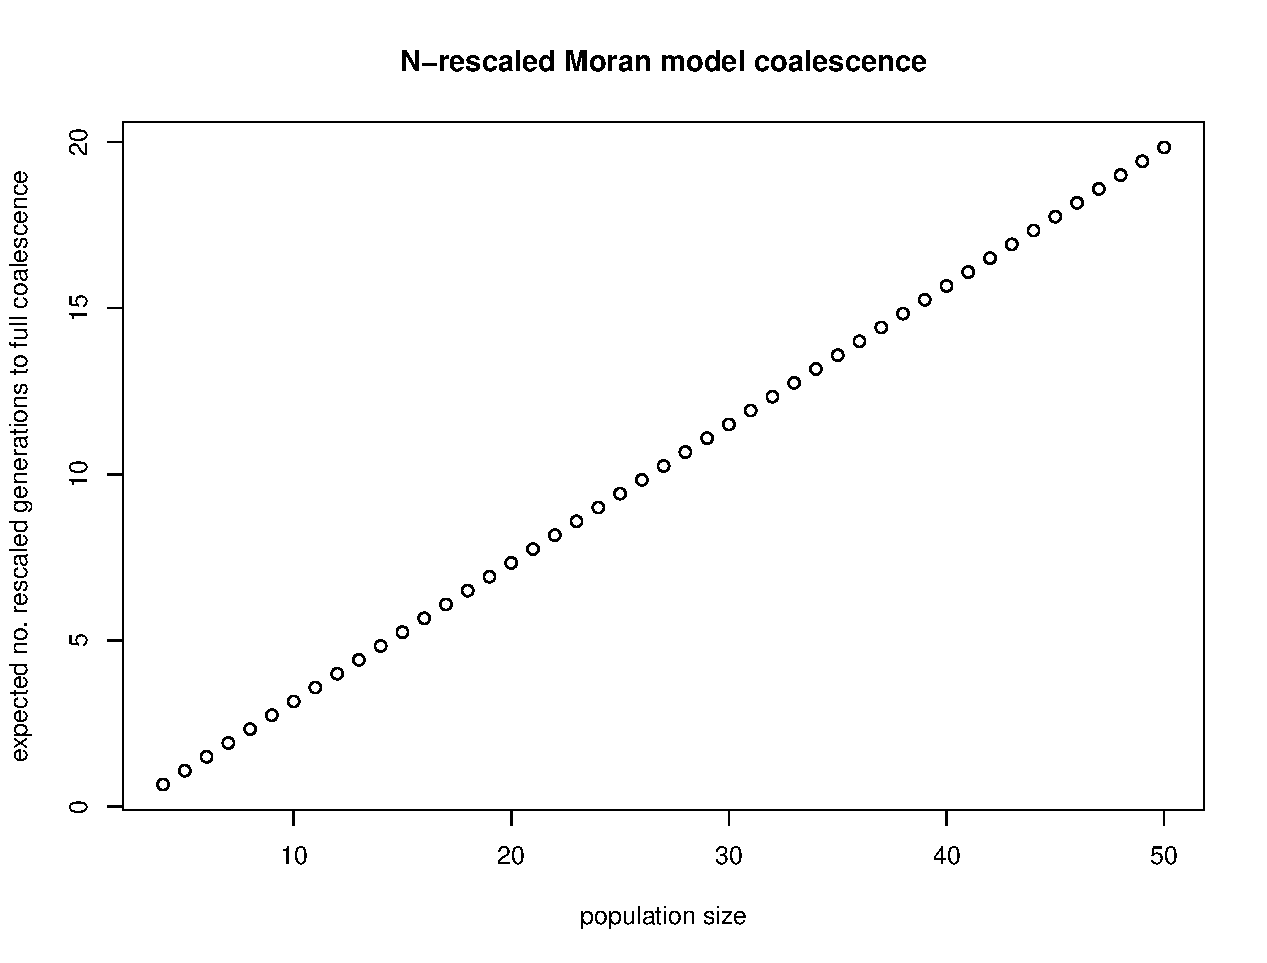
\includegraphics[width=0.5\textwidth]{scalemoran_fullcoal.pdf}\label{fig:scalemoran_fullcoal}}
  \caption{Expected number of generations to full coalescence $\E(\tau)$ in the Moran model, over a range of population sizes $N$. In (b) $\tau$ is measured in rescaled generations (number of generations divided by $N$).}
  \label{fig:moran_coal}
\end{figure}

\subsubsection*{A loose bound}
Let us consider another quantity, $\PR(\tau \leq N)$. This is the probability that $N$ generations back, all $N$ lineages have coalesced. Since at most one pair of lineages can coalesce in one step, we have $\PR(\tau \leq N) = \PR(\tau = N)$.
Now we can put a (seemingly loose, at least for larger $N$) bound on this probability. The event $\{\tau=N\}$ can only happen if there is some pair coalescence in every generation $1,\dots,N$ (regardless of whether it is a useful coalescence). The probability of having no coalescence in a given generation is $1/N$, and is independent between generations. Therefore
\begin{equation*}
\PR(\tau \leq N) = \PR(\tau = N) \leq \left(1-\frac{1}{N}\right)^N \underset{N\rightarrow\infty}{\nearrow} e^{-1} \simeq 0.37
\end{equation*}
Consider this bound in light of the results in Figure \ref{fig:moran_coal}.

\subsubsection*{Distribution of the full coalescence time}
It turns out we can find a closed form (though not a beautiful one) for the full distribution of $\tau$. We divide into three cases for $\PR(\tau=k)$:
\begin{enumerate}
\item $k<N-1$. In this case there have not yet been enough steps to transition from state 0 to state N-1, since we can move up at most one state per step.
\begin{equation*}
\PR(\tau<N-1)=0
\end{equation*}

\item $k=N-1$. The only way to transition from state 0 to state $N-1$ in $N-1$ steps is to move up a state at every step. 
\begin{equation*}
\PR(\tau=N-1) = \prod_{i=0}^{N-2} p_{i,i+1} = \prod_{i=0}^{N-2} \frac{(N-i)(N-i-1)}{N^2}
\end{equation*}

\item $k>N-1$. Now we must make sure we don't arrive in state $N-1$ too early. In order to have $\tau=N-1+M$, we must ``rest'' (remain in the same state) exactly M times. These rests could happen in any $M$ (not necessarily distinct) states $0,\dots,N-2$. Additionally we must at some point make all of the $N-1$ transitions up one state, as in the case $k=N-1$.
\begin{align*}
\PR(\tau=N-1+M) &= \prod_{i=0}^{N-2} p_{i,i+1} \sum_{\substack{i_1,\dots,i_M\\ \in \{0,\dots,N-2\}}} \prod_{j=1}^M p_{i_j,i_j} \\
&= \prod_{i=0}^{N-2} p_{i,i+1} \sum_{\substack{i_1,\dots,i_M\\ \in \{0,\dots,N-2\}}} \prod_{j=1}^M (1-p_{i_j,i_j+1}) \\
&= \prod_{i=0}^{N-2} \frac{(N-i)(N-i-1)}{N^2} \sum_{\substack{i_1,\dots,i_M\\ \in \{0,\dots,N-2\}}} \prod_{j=1}^M \left(1-\frac{(N-i_j)(N-i_j-1)}{N^2}\right)
\end{align*}
\end{enumerate}

\subsection*{Wright-Fisher model}
For the standard Wright-Fisher model (with constant populations size $N$ and exchangeable offspring distributions i.e.\ uniform weights), $\{c_r\}_{r\in\mathbb{N}}$ is again a Markov chain, with transition probabilities given by
\begin{equation}\label{eq:WF_coal_transprob}
p_{i,j} := \PR(c_{r+1} = j \mid c_r =i) = 
\begin{cases}
  1 &\text{if } i=j=N-1 \\
  \frac{S_{N-i}^{(N-j)} (N)_{N-j}}{N^{N-i}} &\text{if } j\geq i;\, i,j=0,\dots,N-2 \\
  0 &\text{otherwise}
\end{cases}
\end{equation}
obtained from \citet[equation 3.12]{wakeley2009} by noting that the number of lineages ``alive'' at generation $r$ is $N-c_r$.
$S_x^{(y)}$ is the number of ways to partition a set of $x$ elements into $y$ non-empty subsets, called Stirling numbers of the second kind (OEIS A008277).

We can now calculate the expectation and variance of $\tau$ numerically as we did for the Moran model.

\section*{Notes from \citet{koskela2018}}
\subsection*{Notation}

\subsection*{}



\bibliography{smc.bib}
\end{document}
